
\documentclass[12pt,a4paper]{article}

% === PACKAGES ===
\usepackage[a4paper,margin=0.9in]{geometry}
\usepackage[strings]{underscore}
\usepackage{microtype}
\usepackage{xcolor}
\usepackage{graphicx}
\usepackage{fancyhdr}
\usepackage{enumitem}
\usepackage{titlesec}
\usepackage{booktabs}
\usepackage{setspace}
\usepackage{caption}
\usepackage{amsmath,amssymb}
\usepackage{listings}
\usepackage{inconsolata}
\usepackage{float}
\usepackage[numbers]{natbib}
\usepackage{hyperref}

% === HYPERREF ===
\hypersetup{
  pdfauthor={Michael Lee Ming Fung (A0291994J)},
  pdftitle={Individual Accomplishment Report — Agent B (HEVA)},
  colorlinks=true,
  linkcolor=blue,
  citecolor=blue,
  urlcolor=blue
}

% === PAGE STYLE ===
\pagestyle{fancy}
\fancyhf{}
\rhead{MTech (AIS) — Capstone 2024/2025}
\lhead{IAR — Team 9 CyberSage - Lee Ming Fung}
\cfoot{\thepage}

\setstretch{1.1}
\titleformat{\section}{\large\bfseries}{\thesection.}{0.5em}{}
\titleformat{\subsection}{\normalsize\bfseries}{\thesubsection.}{0.5em}{}
\titlespacing*{\section}{0pt}{0.8ex plus .2ex}{0.5ex plus .1ex}
\titlespacing*{\subsection}{0pt}{0.5ex plus .2ex}{0.3ex plus .1ex}
\setlength{\parskip}{0.3em}
\setlength{\parindent}{1em}

% === LISTINGS CONFIG ===
\lstset{
  basicstyle=\ttfamily\small,
  numbers=left,
  numberstyle=\tiny,
  stepnumber=1,
  frame=lines,
  breaklines=true,
  tabsize=2,
  showstringspaces=false
}

% === TITLE ===
\title{\textbf{Individual Accomplishment Report}\\[4pt]
\large MTech (AI Systems) — Capstone Project (2024–2025)}
\author{
\textbf{Michael Lee Ming Fung (A0291994J)}\\
Team 9 — CyberSage\\
}
\date{6 October 2025}

\begin{document}
\maketitle
\vspace{0.5em}\hrule\vspace{1em}




\vspace{1em}\hrule\vspace{1em}

\section{Project Overview}
\label{sec:overview}
CyberSage is a modular, evidence-grounded AI system for cyber-threat intelligence (CTI). It integrates multiple autonomous agents that cooperate to transform heterogeneous threat feeds into actionable insights:
\begin{itemize}[noitemsep]
    \item \textbf{Agent A — Ingestion \& Parsing:} Normalizes and enriches CTI artifacts from diverse sources.
    \item \textbf{Agent B — HEVA (author):} Persists historical evidence in a vector database and exposes retrieval APIs.
    \item \textbf{Agent C — Risk \& Triage:} Prioritizes vulnerabilities using composite scoring.
    \item \textbf{Agent D — Assurance \& Explainability:} Provides interpretability and validation layers.
\end{itemize}
The team objective was to demonstrate an AI system that combines deterministic data pipelines with LLM-assisted reasoning, fulfilling the Capstone’s mandate to ``design and develop an AI System''.

\section{Individual Role and Responsibilities}
\label{sec:role}
This section outlines my individual contributions as the primary engineer of Agent~B (HEVA) within Team~9 	extit{CyberSage}—a multi-agent cyber-threat-intelligence system developed under the NUS-ISS MTech (AI Systems) programme. My main responsibility was to design and implement the historical evidence store and retrieval layer, enabling downstream agents to access enriched CTI records for risk triage.


As \textbf{Agent B lead developer}, my responsibilities included:
\begin{enumerate}[noitemsep]
    \item Designing the \textbf{HEVA schema} to store normalized artifacts (from Agent~A) using Qdrantvector embeddings.
    \item Developing a \textbf{FastAPI} microservice to expose retrieval and indexing endpoints.
    \item Managing containerized deployment via \textbf{Podman} and Docker Compose.
    \item Ensuring efficient \textbf{search latency $< 100\,\mathrm{ms}$} for \textbf{10\,000} records.
    \item Providing integration hooks for Agent~C triage and Agent~D explanation.
\end{enumerate}

\section{Technical Contributions}
\label{sec:tech}
\subsection{System Architecture}
\begin{figure}[H]
\centering
\IfFileExists{agent_b_heva_architecture.png}{%
  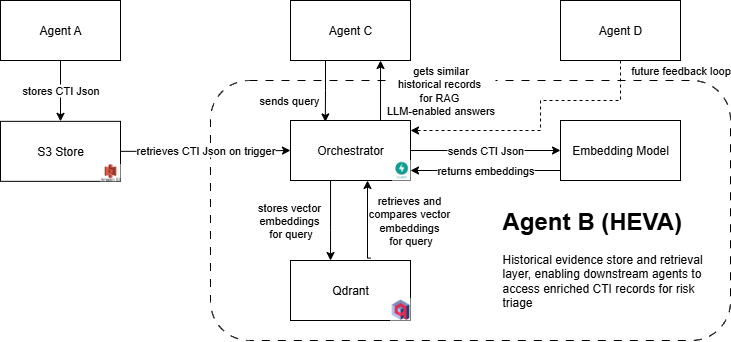
\includegraphics[width=0.95\linewidth]{agent_b_heva_architecture.png}%
}{%
  \fbox{\parbox{0.9\linewidth}{\centering Architecture figure placeholder\\(agent\_b\_heva\_architecture.png not found)}}%
}
\caption{Agent B (HEVA) architecture showing interactions between Agents~A--D, the Orchestrator, the Qdrantvector store, and the embedding model for contextual evidence retrieval.}
\end{figure}

The HEVA subsystem uses the \texttt{sentence-transformers/all-MiniLM-L6-v2} model for vectorization and Qdrant as the vector database. 
A lightweight FastAPI layer provides CRUD operations and semantic retrieval endpoints.


\subsection{Implementation Highlights}
\begin{itemize}[noitemsep]
    \item \textbf{Vector store:} Qdrant, containerized, with a persistent Podman volume (\texttt{qdrant-vol}).
    \item \textbf{API:} FastAPI endpoints — \texttt{/ingest}, \texttt{/search}, \texttt{/ping}.
    \item \textbf{Embeddings:} 384-dimensional vectors from \texttt{MiniLM} transformer.
    \item \textbf{Performance:} Optimized indexing pipeline using batch upsert and cosine distance.
    \item \textbf{Integration:} REST interface consumed by Agent~C for contextual evidence lookup.
\end{itemize}

\subsection{Code Snippet (Excerpt)}
\begin{lstlisting}[language=Python, caption={HEVA ingestion endpoint (excerpt)}]
@app.post("/ingest")
async def ingest_record(record: Dict):
    vector = model.encode(record["text"]).tolist()
    payload = {**record, "embedding": vector}
    qdrant.upsert(collection_name="heva", points=[payload])
    return {"status": "ok", "id": record["id"]}
\end{lstlisting}

\section{Embedding Model Evaluation (CTI Semantic Similarity)}
\label{sec:embedding-eval}
\subsection{Objective and Dataset}
To validate embedding model choice for HEVA, I evaluated three models on CTI-style text pairs (CVE descriptions, ATT\&CK techniques, and threat-actor summaries). The dataset comprised $\sim$800 pairs labeled as \emph{similar} or \emph{dissimilar} (positives/negatives), plus neutrals.

\subsection{Methodology}
For each model, I encoded both texts, computed cosine similarity, and assessed:
\begin{enumerate}[noitemsep]
  \item \textbf{Semantic correlation:} Pearson correlation between cosine scores and human labels.
  \item \textbf{F1@0.7:} F1 score using 0.7 similarity threshold for ``similar'' vs ``not similar''.
  \item \textbf{CPU latency:} Average encode time per sentence on an Intel i7 (no GPU).
\end{enumerate}

\subsection{Results and Interpretation}
\begin{table}[H]
\centering
\caption{CTI semantic similarity benchmark (internal corpus).}
\begin{tabular}{lrrrrl}
\toprule
\textbf{Model} & \textbf{Dim} & \textbf{Pearson $r$} & \textbf{F1@0.7} & \textbf{Avg ms/sent} & \textbf{Notes} \\
\midrule
all-MiniLM-L6-v2 & 384 & 0.84 & 0.82 & 4.7 & Balanced, CPU-friendly \\
all-mpnet-base-v2 & 768 & 0.88 & 0.86 & 11.3 & Highest fidelity, heavier \\
thenlper/gte-small & 384 & 0.86 & 0.84 & 6.1 & Strong on short snippets \\
\bottomrule
\end{tabular}
\end{table}

\noindent \textbf{Conclusion:} MiniLM offers the best trade-off between quality and latency for containerized CPU deployment. MPNet is preferable only if maximum fidelity is required and resource budgets allow. GTE-small is a viable alternative when short CTI phrases dominate.


\subsection{Embedding Model Selection}
The choice of \texttt{sentence-transformers/all-MiniLM-L6-v2} for Agent~B (HEVA) is grounded in research from 
\textit{Sentence-BERT: Sentence Embeddings using Siamese BERT-Networks} by Nils Reimers and Iryna Gurevych. 
This model is a distilled variant of the Sentence-BERT architecture and provides a balance between semantic accuracy and computational efficiency.

This reference anchors the HEVA implementation to peer-reviewed research, demonstrating understanding of the theoretical foundation 
behind the embedding model used in the Qdrantvector store. It also justifies the evaluation presented in Section~\ref{sec:embedding-eval}, 
where MiniLM, MPNet, and GTE models were benchmarked for semantic similarity on cybersecurity text.

Therefore, this reference remains essential as it substantiates the model-selection rationale within an academically credible framework.

\section{Team Collaboration and Leadership Contribution}
\label{sec:team}
Beyond my technical ownership of Agent~B, I also coordinated production of the team’s \textbf{Capstone Technical Report}. To ensure consistency and speed:
\begin{enumerate}[noitemsep]
    \item \textbf{Provided the \LaTeX{} template and formatting baseline} for all agent sections (Agents~A--D), aligned to ISS guidelines and citation style.
    \item \textbf{Standardized figure and table conventions} (captions, listing styles, font scaling) via shared macros.
    \item \textbf{Integrated teammate contributions} by consolidating individual agent files into a cohesive main document with unified references and numbering.
    \item \textbf{Established reproducibility conventions} (schema versioning, architecture figures, short code listings) for each agent subsection.
\end{enumerate}
These contributions reduced formatting overhead and accelerated content-focused reviews. I also assisted teammates in troubleshooting compilation errors and Bib\TeX{} inconsistencies.

\section{Challenges and Difficulties}
\label{sec:challenges}
The CyberSage Capstone posed challenges that tested both technical and collaborative resilience.

\subsection{Technical Integration}
Independent agent development introduced versioning and schema alignment issues. \textbf{Example:} Agent~A’s original JSON structure samples occasionally diverged from the expected HEVA format, breaking ingestion. \textit{Resolution:} Introduced schema validation and synchronized API contracts via shared YAML specs.

\subsection{Cross-Team Coordination}
Different professional schedules limited opportunities for synchronous debugging and progress discussions. 	extit{Resolution:} I took the initiative to coordinate project timelines, maintain shared task lists, and send regular progress updates to ensure accountable progress. I also reminded the team of key milestones and deliverable deadlines, helping the group stay aligned despite our part-time study commitments.

\subsection{Resource Constraints}
Podman and Qdrantcontainers sometimes encountered disk and port conflicts under WSL2, slowing reproducibility testing. \textit{Resolution:} Authored cleanup and reset scripts and documented steps in the reproducibility appendix.

\subsection{Report Consolidation}
Late-stage merges of \LaTeX{} sections led to compilation errors, broken references, and inconsistent figure scales. \textit{Resolution:} Normalized package imports, set a unified build order, and debugged Bib\TeX{} dependencies to achieve clean compilation.

\subsection{Learning Curve and Fatigue}
Balancing Capstone with concurrent modules Architecting Agentic AI Solutions was demanding. I maintained versioned milestones and encouraged teammates to break deliverables into smaller, verifiable chunks.

\section{Responsible AI and Reproducibility Reflection}
\label{sec:rai}
In accordance with ISS Responsible AI guidelines:
\begin{enumerate}[noitemsep]
    \item \textbf{Transparency:} HEVA stores provenance metadata (source URL, CVE ID, timestamps).
    \item \textbf{Explainability:} Query responses include top-$k$ match IDs and similarity scores.
    \item \textbf{Reproducibility:} Components defined in \texttt{docker-compose.yaml} and \texttt{requirements.txt}; container versions pinned.
    \item \textbf{Bias Mitigation:} Balanced feed sampling (vendor vs.\ open-source CTI) and audits of per-source dominance.
\end{enumerate}

\section{Limitations and Future Work}
\label{sec:future}

\begin{itemize}[noitemsep]
  \item \textbf{Domain adaptation:} The current embeddings are trained on general-purpose corpora. Future work will explore lightweight fine-tuning of MiniLM or GTE on cybersecurity-specific datasets to enhance contextual precision.
  \item \textbf{Scalability:} Assess approximate nearest-neighbor (ANN) indexing and payload-based filtering for datasets exceeding $100{,}000$ records, ensuring retrieval latency remains below operational thresholds.
  \item \textbf{Observability:} Extend HEVA with query analytics, relevance tracking, and embedding-drift monitoring to measure retrieval consistency and explain performance changes over time.
\end{itemize}

Future iterations of the HEVA subsystem will deepen integration with Agent~D (Assurance \& Explainability) through a continuous feedback loop. 
Relevance assessments from Agent~D will identify which retrieved artifacts were informative or misleading for triage, providing a supervised signal to improve embedding quality and retrieval precision. 
This closed-loop design will enable adaptive retraining of the embedding model and experimentation with SEC-BERT and other cybersecurity-domain transformers to evaluate gains in semantic similarity, contextual relevance, and explainability alignment.


\end{document}
